% !TeX encoding = UTF-8
% !TeX program = xelatex
% !TeX spellcheck = en_US

\documentclass[degree=project,degree-type=project,cjk-font=noto]{thuthesis}
\usepackage{mathtools}
\usepackage{tikz}
\usetikzlibrary{shapes,arrows}
\usepackage[autosize]{dot2texi}
% Syntax Highlighting in LaTeX, need pygments
% Must build with xelatex -shell-escape -enable-8bit-chars.
\usepackage{minted}
% https://tex.stackexchange.com/a/112573
\usepackage{tcolorbox}
\usepackage{etoolbox}
\BeforeBeginEnvironment{minted}{\begin{tcolorbox}}%
\AfterEndEnvironment{minted}{\end{tcolorbox}}%
% color for minted
\definecolor{friendlybg}{HTML}{f0f0f0}


% 论文基本配置,加载宏包等全局配置
\thusetup{
    output = electronic,
    title  = {实验三:基于PPG的语音转换系统},
    author  = {肖文韬},
    studentid = {2020214245},
    major = {电子信息(计算机技术)},
    email = {xwt20@mails.tsinghua.edu.cn},
    course = {语音信号数字处理},
    include-spine = false,
}


\usepackage{float}
\usepackage[sort]{natbib}
\bibliographystyle{thuthesis-numeric}
\graphicspath{{figures/}}


\begin{document}

% 封面
\maketitle

\frontmatter
% % !TeX root = ../thuthesis-example.tex

% 中英文摘要和关键字

\begin{abstract}
  论文的摘要是对论文研究内容和成果的高度概括。摘要应对论文所研究的问题及其研究目
  的进行描述,对研究方法和过程进行简单介绍,对研究成果和所得结论进行概括。摘要应
  具有独立性和自明性,其内容应包含与论文全文同等量的主要信息。使读者即使不阅读全
  文,通过摘要就能了解论文的总体内容和主要成果。

  论文摘要的书写应力求精确、简明。切忌写成对论文书写内容进行提要的形式,尤其要避
  免“第 1 章……;第 2 章……;……”这种或类似的陈述方式。

  本文介绍清华大学论文模板 \thuthesis{} 的使用方法。本模板符合学校的本科、硕士、
  博士论文格式要求。

  本文的创新点主要有:
  \begin{itemize}
    \item 用例子来解释模板的使用方法;
    \item 用废话来填充无关紧要的部分;
    \item 一边学习摸索一边编写新代码。
  \end{itemize}

  关键词是为了文献标引工作、用以表示全文主要内容信息的单词或术语。关键词不超过 5
  个,每个关键词中间用分号分隔。(模板作者注:关键词分隔符不用考虑,模板会自动处
  理。英文关键词同理。)

  % 关键词用“英文逗号”分隔
  \thusetup{
    keywords = {TeX, LaTeX, CJK, 模板, 论文},
  }
\end{abstract}

\begin{abstract*}
  An abstract of a dissertation is a summary and extraction of research work
  and contributions. Included in an abstract should be description of research
  topic and research objective, brief introduction to methodology and research
  process, and summarization of conclusion and contributions of the
  research. An abstract should be characterized by independence and clarity and
  carry identical information with the dissertation. It should be such that the
  general idea and major contributions of the dissertation are conveyed without
  reading the dissertation.

  An abstract should be concise and to the point. It is a misunderstanding to
  make an abstract an outline of the dissertation and words ``the first
  chapter'', ``the second chapter'' and the like should be avoided in the
  abstract.

  Key words are terms used in a dissertation for indexing, reflecting core
  information of the dissertation. An abstract may contain a maximum of 5 key
  words, with semi-colons used in between to separate one another.

  \thusetup{
    keywords* = {TeX, LaTeX, CJK, template, thesis},
  }
\end{abstract*}


% 目录
\tableofcontents

% 插图和附表清单
\listoffiguresandtables
% \listoffigures           % 插图清单

% 正文部分
\mainmatter

\chapter{任务一: 提取 PPG 与声学参数 ($15"$)}

\section{任务介绍}

为了进行语音转换,我们首先需要使用 ASR 系统将源音频转换为一种中间特征(在本实验中就是音素序列 PPG~\cite{PPG}),对每一帧的 MFCC 特征 $X_t$ 我们可以得到所有音素(音素集 $\mathcal{S}$)的后验概率 $\{p(s | X_t) | s \in \mathcal{S}\}$。
同时,我们还可以将原始波形序列加窗得到语音帧,对语音帧进行离散傅里叶变换后,计算各频率分量的能量后可以得到语谱图(线性谱)。
而我们知道人类对低频成分更加敏感,而对高频不敏感,所以我们取对数后可以得到对应的 Mel 谱。
本任务就是使用预训练模型得到音频的 PPG,同时还需要计算得到基频 $F_0$, 线性谱,Mel 谱等声学参数。

接下来的小节就是回答问题啦。

\section{提取音素后验概率 PPG ($4"$)}

\textbf{(1) 简要说明 PPG 提取器(ppg\_extractor)的网络结构,给出网络的基本结构图。}

\begin{figure}[!htp]
\centering%
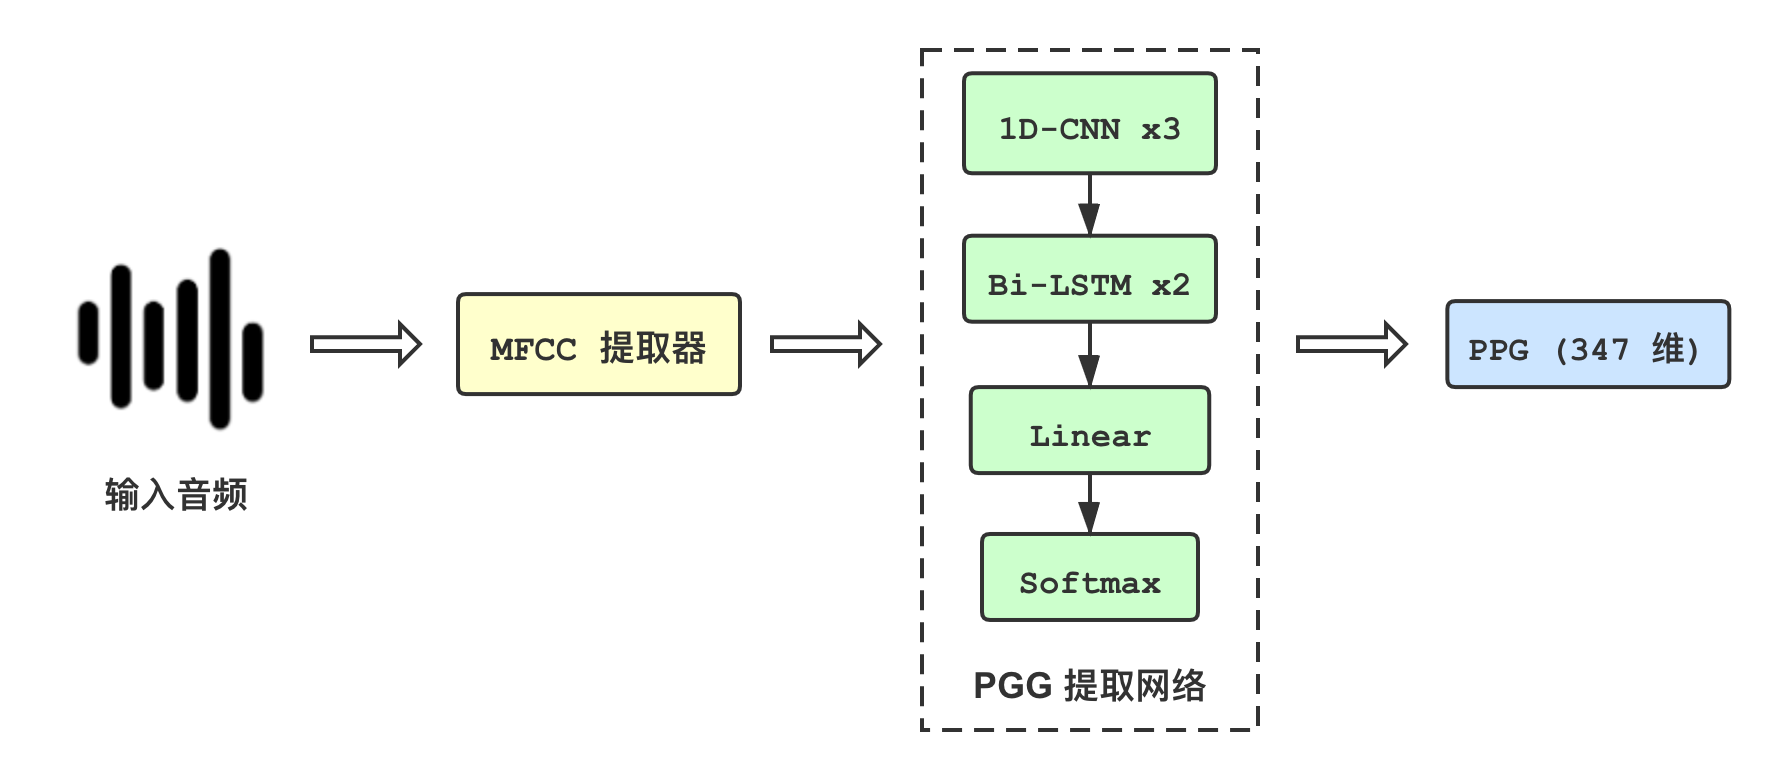
\includegraphics[width=.8\linewidth]{PPG.png}
  \caption{PPG 提取流程图}
  \label{fig:ppg}
\end{figure}


\textbf{答}: PPG 提取器网络由卷积层、LSTM 和线性层组成,具体组成如图~\ref{fig:ppg}所示。

\section{理解 Mel 谱等声学参数的提取过程($3" + 3"$)}

(2) 理解声学参数提取的过程,为 hparam.py 中 class Audio 的主要参数添加注释,说
明该参数的意义,可在实验报告中截图或者表格展示。

\begin{table}[htb]
  \centering
  \caption{class Audio 主要参数说明}
  \label{tab:audio_param}
  \begin{tabular}{cc}
    \toprule
    \textbf{参数}         & \textbf{说明}  \\
    \midrule
    \texttt{num\_mels = 80} & Mel 谱的数量\\
    \texttt{ppg\_dim = 347} & PPG 特征维度 \\
    \texttt{num\_freq = 1025} & 频率数目 \\
    \texttt{min\_mel\_freq = 30} & Mel 谱的最低频率 \\
    \texttt{max\_mel\_freq = 7600} & Mel 谱的最高频率 \\
    \texttt{sample\_rate = 16000} & 采样率 \\
    \texttt{frame\_length\_ms = 25} & 窗长(单位ms) \\
    \texttt{frame\_shift\_ms = 10} & 窗移(单位ms) \\
    \texttt{upper\_f0 = 500} & 基频 $F_0$ 上限 \\
    \texttt{lower\_f0 = 30} & 基频 $F_0$ 下限 \\
    \midrule
    \texttt{n\_mfcc = 13} & mfcc 特征的数量 \\
    \texttt{preemphasize=0.97} & preemphasisi滤波系数 \\
    \texttt{min\_level\_db = -80.0} & 最小 level 的响度(单位dB) \\
    \texttt{ref\_level\_db = 20.0} & 相对 level 的响度(单位dB) \\
    \texttt{max\_abs\_value = 1.} & 最大的绝对值 \\
    \texttt{symmetric\_specs = False} & 语谱图是否对称 \\
    \texttt{griffin\_lim\_iters = 60} & griffin-lim 滤波器的迭代次数 \\
    \texttt{power = 1.5} & 能量 \\
    \texttt{center = True} & 是否中心化 \\
    \bottomrule
  \end{tabular}
\end{table}

参数说明如表\ref{tab:audio_param}所示。

\section{提取 Mel 谱等声学参数($6"$)}

\textbf{(3)Mel 谱和线性谱的提取过程有什么差异?它们之间是什么关系?}

\textbf{答:} Mel 谱就是将线性频谱取对数映射至 Mel 刻度上。
将原始波形序列加窗得到语音帧,对语音帧进行离散傅里叶变换后,计算各频率分量的能量后可以得到语谱图(线性谱)。
而我们知道人类对低频成分更加敏感,而对高频不敏感,所以我们取对数后可以得到对应的 Mel 谱。

\textbf{(4)提取出来的线性谱和 Mel 谱各是多少维的特征参数?Mel 谱的频率范围是多少?}

\textbf{答:}
线性谱 $1025$,Mel 谱 $80$。Mel 谱的频率范围为 $30 \sim 7600$Hz.

\textbf{(5)基频参数 log(F0)的提取经过了什么样的操作,为什么要这样操作?在语音转换中 PPG 提供了语言内容信息,基频参数 log(F0)提供了什么信息?}

\textbf{答:}

处理代码在 \texttt{utils/audio.py:47}:
  \begin{minted}[texcomments,tabsize=2,fontsize=\footnotesize,style=friendly,bgcolor=friendlybg]{python}
val1 = subprocess.call('sox {} -t raw {}'.format(wav_path, temp_raw_path), shell=True)
val2 = subprocess.call('x2x +sf {} | pitch -H {} -L {} -p {} -s {} -o 2 > {}'.format(
	temp_raw_path, upper_f0, lower_f0, hop_len, fs_khz, save_path), shell=True)
  \end{minted}

主要就是使用 sox 提取 wav 文件的音频波心的 Raw 文件。
然后使用 x2x 将类型从 short 转化为 float,在用 pitch 提取出 $\log(F_0)$。
基频参数 $\log(F_0)$ 提供的是说话人的声门波的基频。

\section{数据集的划分($2"$)}

\textbf{(6)实验中将数据集划分为了训练集、验证集、测试集。它们之间的默认划分比例是 多少?}

\textbf{答:}
训练集,验证集,测试集分别占 90\%,5\%,5\%。

\chapter{任务二: 训练并测试特定目标说话人的语音转换模型($40"$)}

基于任务一提取出的音素后验概率 PPG 和 Mel 谱的数据,将其作为 PPG 到 Mel 谱映射 模型(Conversion Model)的输入和输出,训练该映射模型至收敛;并进而利用训练好的模 型进行测试和语音转换。
训练日志保存在 \texttt{logs/train\_task2.log}

\section{数据集及数据加载模块定义($5"$)}

\textbf{(1)了解 DataSet 及 VCDataSet 类的原理,熟悉 DataLoader 类调用时各参数的含义。 在实验报告中回答 DataLoader 的调用参数 batch\_size、shuffle、num\_workers、collate\_fn 分 别是什么含义?}

\textbf{答:}
DataSet 类是 PyTorch 提供的一个用于实现数据集的类,用户如果需要实现自己的数据集类型,只需要继承 DataSet 类,然后覆写 \texttt{\_\_getitem\_\_} 和 \texttt{\_\_len\_\_} 两个方法即可。
VCDataset 类就是 DataSet 的子类,其提供了根据样本序号,提取出的语音数据集的样本的功能,每个样本包含了fid, ppg, mel, linear, log\_f0 这五个数据。

DataLoader 的调用参数含义:

\begin{enumerate}
	\item \textbf{batch\_size}:表示数据批次的大小,因为训练我们采用的是 mini batch,也就是每次只训练数据集中的一小部分,这一小部分包含的样本数就是 batch size。
	\item \textbf{shuffle}: 表示在读取数据集的时候是否会进行随机打乱顺序,一般为了保证训练结果都建议开启。
	\item \textbf{num\_workers}: 表示读取数据的时候的子进程数,多个子进程有利于加快读取速度。值得一提的是如果在 docker 环境,默认的 num\_workers 参数会导致错误,这是因为 docker 限制了共享内存(shm)的大小。
	\item \textbf{collate\_fn}: 用于控制同一个 batch 的样本如何组成一个 batch,差不多就是一个 filter,因为同一个 batch 里面不同样本的长度可能不一样,需要对他们进行 padding 等操作,才能组成一个合法的 batch。
\end{enumerate}

\section{转换模型定义($8"$)}

\textbf{(2)阅读 train\_to\_one.py,找出转换模型的定义,并根据 models/model.py 说明转换模型的网络结构,给出网络的基本结构图。}

\textbf{答:}

转换模型为 BLSTMConversionModel,其定义为:

  \begin{minted}[texcomments,tabsize=2,fontsize=\footnotesize,style=friendly,bgcolor=friendlybg]{python}
class BLSTMConversionModel(nn.Module):
    """
    Conversion model based on BLSTM
    """
    def __init__(self, in_channels, out_channels, lstm_hidden):
        """
        :param in_channels: input feature dimension,
                            usually (ppg_dim + log-f0s_dim) when
                            use ppgs and log-f0s as inputs
        :param out_channels: mel dimension or your acoustic feature dimnesion
        :param lstm_hidden: parameter dimension
        """
        pass
\end{minted}

\begin{figure}[h]
\centering%
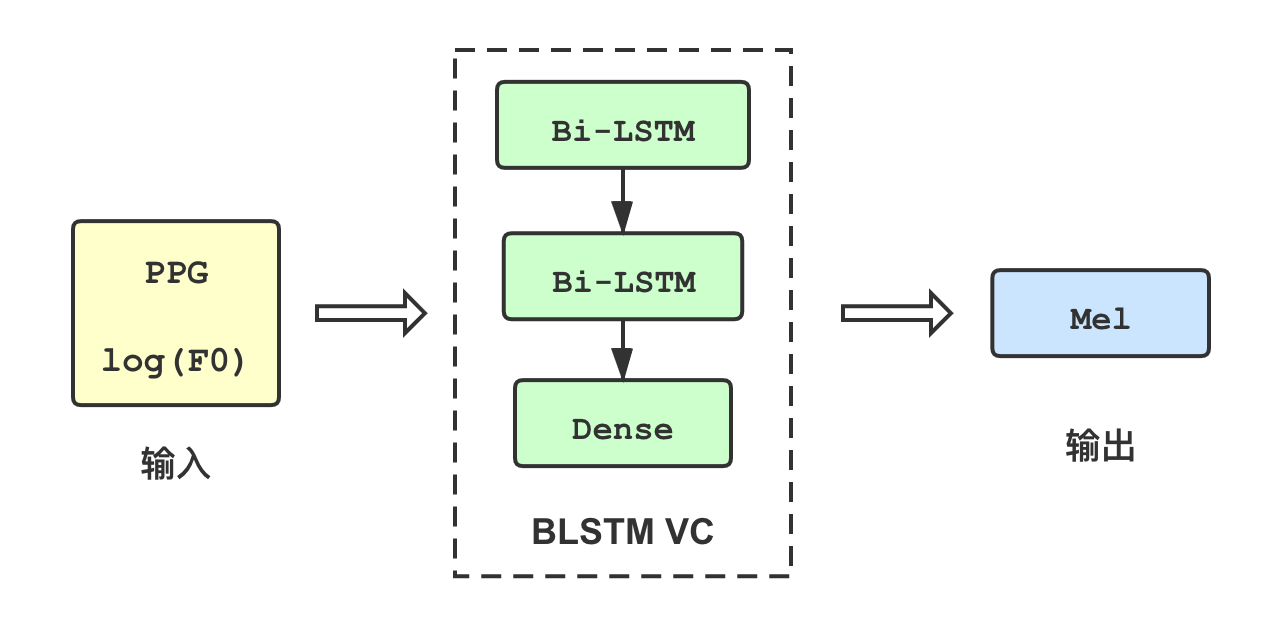
\includegraphics[width=.75\linewidth]{BLSTM_VC.png}
  \caption{Task2 验证集损失图}
  \label{fig:BLSTM_VC}
\end{figure}

图\ref{fig:BLSTM_VC}给出了该模型的网络结构,就是两层双向 LSTM 再加一层全连接层。


\textbf{(3)进而说明转换模型的输入、输出参数分别是什么?输入、输出参数的维数是多少?}

\textbf{答:}

如图\ref{fig:BLSTM_VC}所示,该模型的输入为 PPG 和 log(F0) 拼接而成的特征向量,输出为目标的 Mel 谱。
输入参数的维度为 349 (PPG 的维度为 347, 再加上增加基频特征),输出参数的维度为 80(即 Mel 谱的维度)。

\section{转换模型训练($12"$)}

\textbf{(4)说明转换模型的训练过程,如何进行前向计算?使用了什么损失函数?损失函数是怎么计算的?如何进行误差反向传播?}

\textbf{答:}

1. 训练过程:

\begin{enumerate}
	\item 初始化模型参数
	\item 前向计算,从输入PPG 和 log(F0),输出 Mel 谱
	\item 计算损失函数,计算模型输出的 Mel 谱与实际的 Mel 谱之间的 MSE
	\item 根据损失函数对输入求梯度来反向传播计算所有参数的梯度
	\item 按照梯度信息,以及学习率等超参数,使用制定的优化器进行梯度下降优化,更新参数,并用更新后的参数进入下一轮前向计算,直到收敛
\end{enumerate}

2. 前向计算的方法:

\begin{enumerate}
	\item PPG 和 log(F0) 拼接而成输入 $\bm{x}$
	\item $\bm{x}$ 进入第一层双向 LSTM 得到 \texttt{blstm1\_out}
	\item \texttt{blstm1\_out} 进入第二层双向 LSTM 得到 \texttt{blstm2\_out}
	\item \texttt{blstm2\_out} 进入全连接层得到最终模型输出 \texttt{outputs},这就是模型预测出来的 Mel 谱
\end{enumerate}

3. 损失函数:

带 mask 的 MSE。

因为 batch 中不同样本的长度不一样,而 batch 中因为要构成一个张量,所以我们需要把所有样本填充成相同的长度(这个长度就是最大样本程度)。
但是在计算损失值的时候,我们不需要那些被填充的元素参与到计算,所以我们要通过他们原始的长度信息计算出一个 mask 矩阵。
假定 batch 有 $N$ 个样本,每个样本的长度为 $L = [l_1, \cdots, l_N]$,batch 的形状便是 $(N, \max(L), D)$,mask 矩阵的形状为 $(N, \max(L))$,对于每一行 $[1, \cdots, 1, 0, \cdots, 0]$代表一个样本中每一个时间步是否是被填充的,如果是的话就为 $0$,这样被填充的内容就不会参与到计算中了。

4. 损失函数计算公式:

假设 batch 的计算结果为 $\hat{Y}$,而实际值为 $Y$,mask 矩阵为 $M$(指示矩阵),则带 mask 的 MSE 计算公式为:

\begin{equation}
	\text{MSE} = \frac{N \max(L)}{\sum_i L_i} \lVert M \odot (\hat{Y} - \hat{Y}) \rVert
\end{equation}
其中 $\odot$ 表示逐位乘法($M$ 会 expand 第三维以保持跟 $Y$ 形状一致),$\lVert \cdot \rVert$ 表示先将张量展平为向量在计算其 L2 范数。

5. 误差反向传播:

由 PyTorch 自动完成,其实简单理解就是链式法则来求偏导。

\textbf{(5)给出模型训练时的损失函数曲线;模型训练了多少个 epoch?训练完成后,最终 (对应最后一个 epoch)的平均训练 MSE loss 是多少?}

\begin{figure}[h]
\centering%
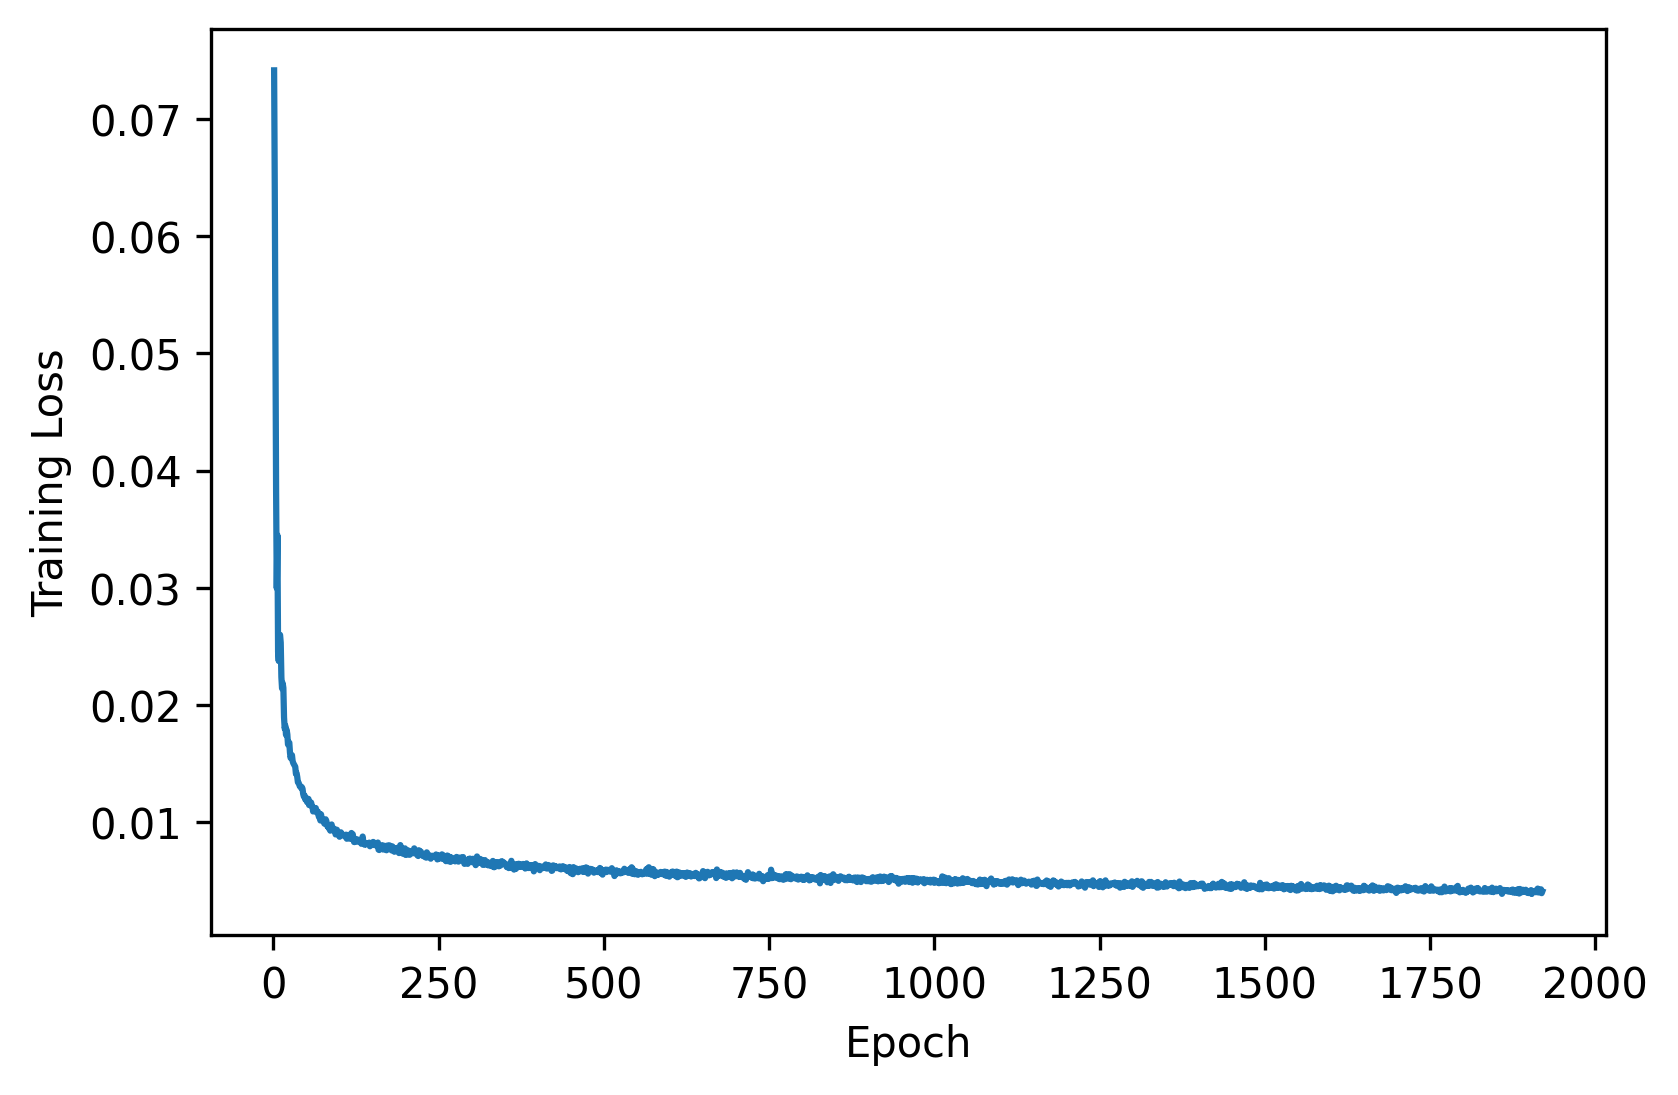
\includegraphics[width=.75\linewidth]{task2_train.png}
  \caption{Task2 训练集损失图}
  \label{fig:task2_train}
\end{figure}

模型训练时的损失函数曲线如图 \ref{fig:task2_train} 所示。

模型总共训练了 60 个 epoch。

最终的平均 MSE loss 为 $0.00410$。

\section{转换模型验证($4"$)}

\textbf{(6) 模型训练的结果保存在什么地方?}

\textbf{答:}
模型保存在由参数 \texttt{args.model\_dir} 指定的目录,默认就是 \texttt{./model\_dir/},命名方式为 \texttt{ppg-vc-to-one-\{\}},\{\} 表示代数。

\textbf{(7)基于上述训练好的模型,在验证集上进行验证。在验证集上的 MSE loss 是多少?}

\textbf{答:}

\begin{figure}[h]
\centering%
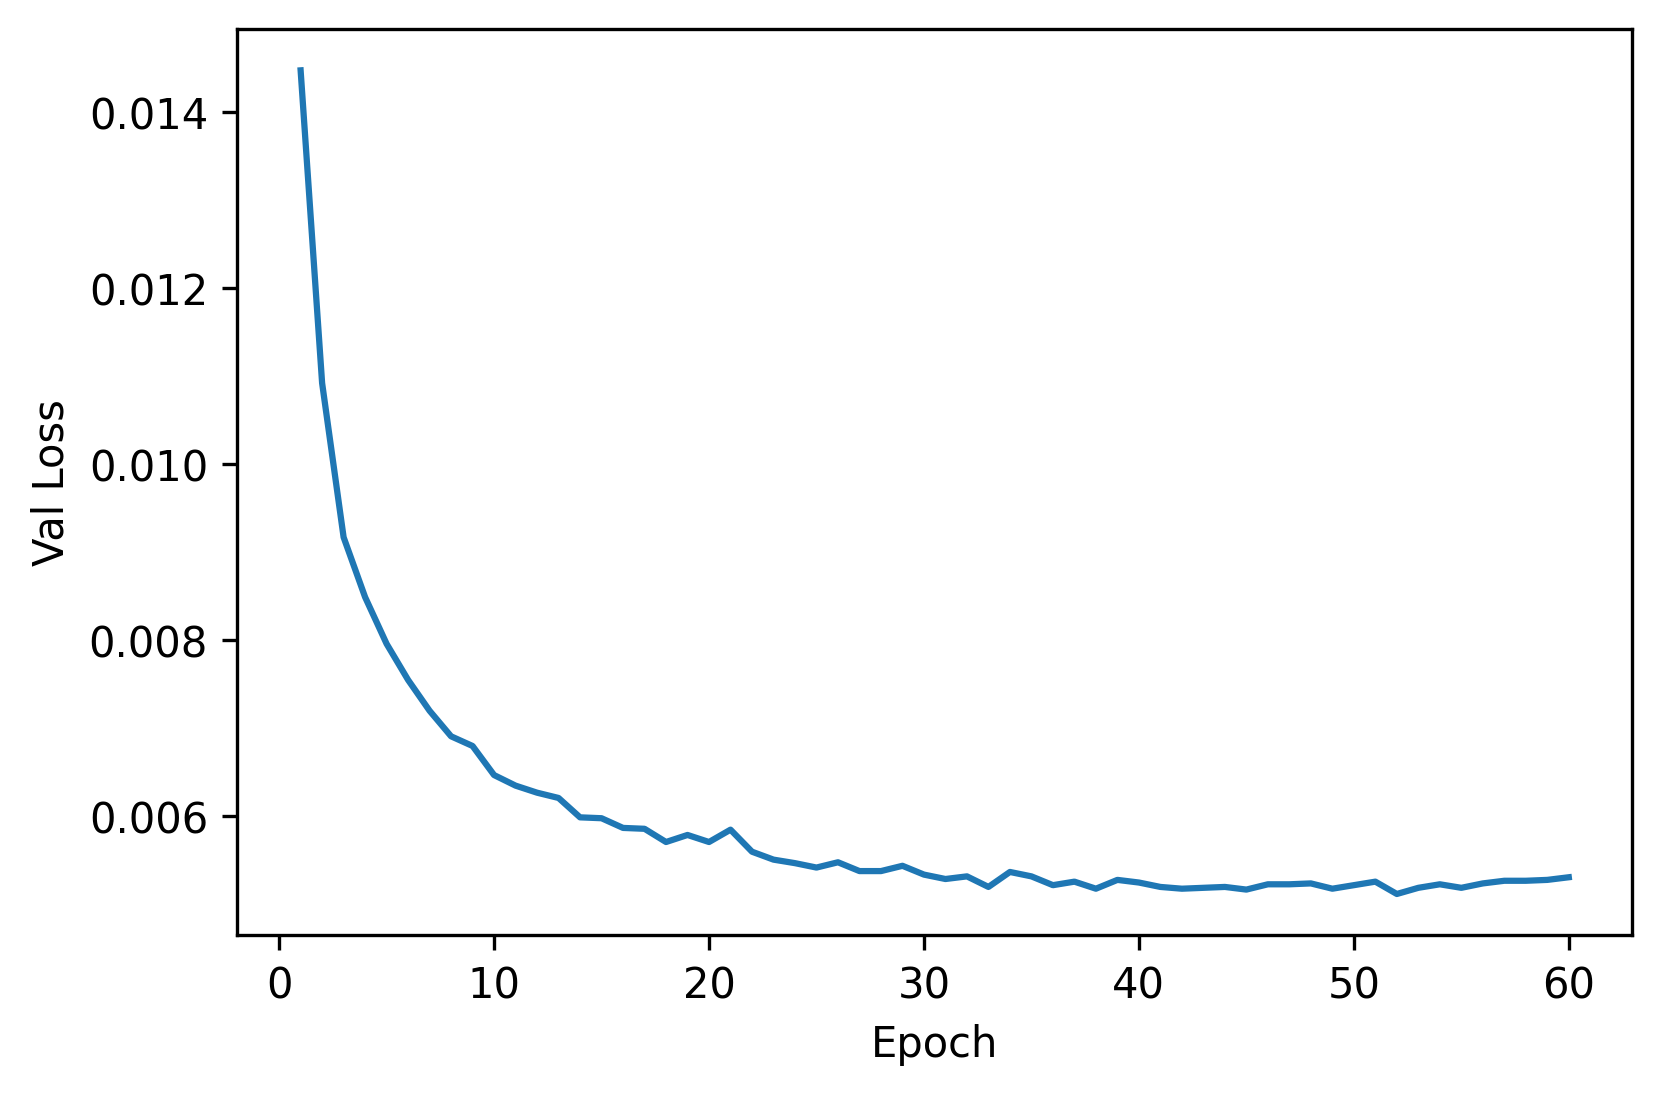
\includegraphics[width=.75\linewidth]{task2_val.png}
  \caption{Task2 验证集损失图}
  \label{fig:task2_val}
\end{figure}

如图\ref{fig:task2_val}所示,在最后一代的验证集 MSE loss 为 $0.00531$。


\section{转换模型测试($5"$)}

\textbf{(8)基于上述训练好的模型,在测试集上进行测试。针对某句测试用例,得到该用例的真实语音以及预测的转换语音;给出该测试用例的真实 Mel 谱、预测 Mel 谱的图,简单 分析它们之间的区别,并计算这两个 Mel 谱之间的均方差 MSE 距离。}

\textbf{答:}
选择 \text{slt\_a0196-56} 作为对比。

\begin{figure}
  \centering
  \subcaptionbox{预测 Mel 谱\label{fig:task2_predicted}}
    {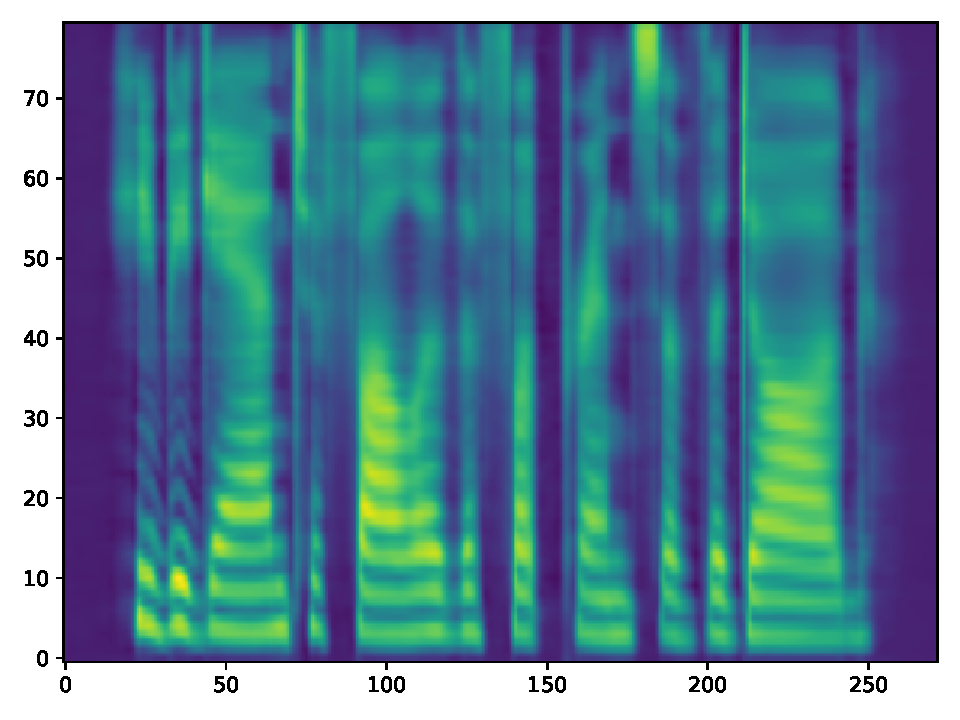
\includegraphics[width=0.45\linewidth]{task2_predicted.pdf}}
  \subcaptionbox{实际 Mel 谱\label{fig:task2_ground}}
    {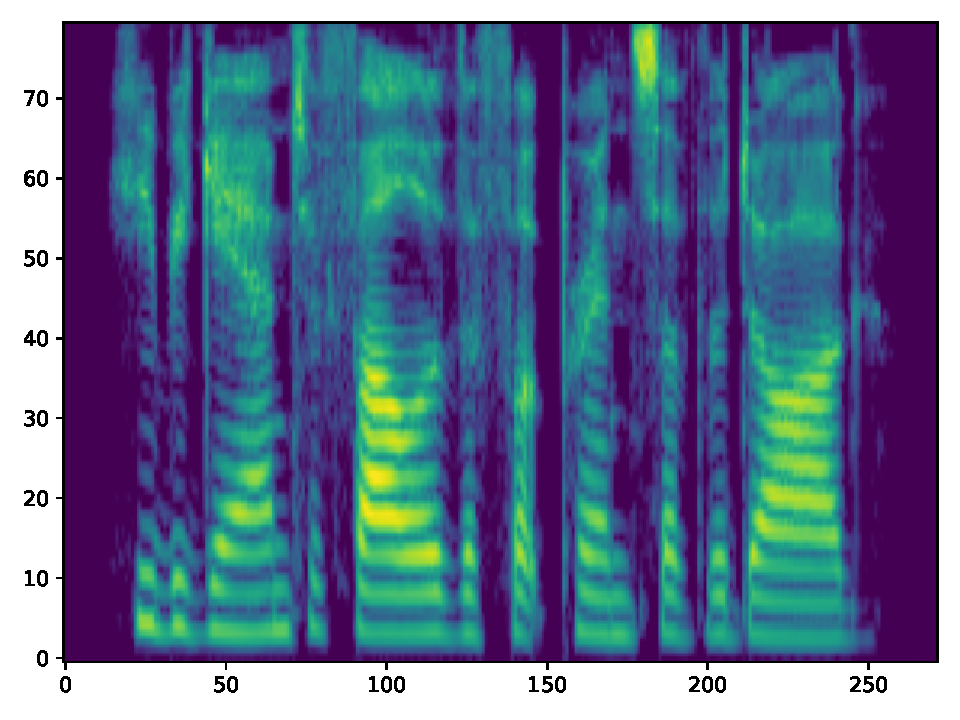
\includegraphics[width=0.45\linewidth]{task2_ground.pdf}}
  \caption{多个分图的示例}
  \label{fig:task2_mel}
\end{figure}

预测和实际 Mel 谱如图 \ref{fig:task2_mel} 所示,可以看到真实的 Mel 谱不同的共振峰之间的界限更加清晰,而预测的 Mel 谱包括基频在内,不同共振峰时间的界限都比较模糊。
最后计算得出两者的 MSE 为 $0.0057$。

\textbf{(9)分析 synthesize\_and\_save\_wavs 所调用的 inv\_mel\_spectrogram 函数,说明将 Mel 谱恢复为语音波形(Speech Waveform)的基本过程,理解声码器(Vocoder)的作用。在实验报告中只需给出 inv\_mel\_spectrogram 函数的流程,说明其所调用的各个子函数的基本功能,不需要深入到子函数中。}

\textbf{答:}

1. inv\_mel\_spectrogram 函数的流程

\begin{enumerate}
	\item 使用\_denormalize()函数将 Mel 谱反标准化
	\item 加上基础的dB,调用\_db\_to\_amp()将dB转化为振幅
	\item 转换为线性谱
	\item 用Griffin-Lim声码器将线性谱转换为语音波形
\end{enumerate}

2. 将 Mel 谱恢复为语音波形(Speech Waveform)的基本过程

声码器用于将声学参数(例如 Mel 谱)转换为语音波形。
因为 Mel 谱只含有幅度谱而重建语音波形缺少相位谱。
Griffin-Lim 就是一种简单高效的声码器,它的核心思想就是用不同帧之间的关系来估计相位。
其工作过程为:

\begin{enumerate}
	\item 初始化一个随机的相位谱
	\item 用这个相位谱与已知的幅度谱(Mel谱)经过傅里叶逆变换合成新的语音波形
	\item 用合成的语音波形经过傅里叶变换,得到新的相位谱和幅度谱
	\item 利用新的相位谱和已知的Mel谱合成新的语音波形
	\item 重复迭代上述步骤多次直到收敛或达到最大迭代次数
\end{enumerate}

\section{进行语音转换($6"$)}

\textbf{(10)结合 inference\_to\_one.py,说明转换阶段由输入源说话人的语音到输出特定目标说话人语音的整体流程。}

\textbf{答:}

流程:

\begin{enumerate}
	\item 将输入 wav 音频文件提取出语音波形
	\item 对语音波形加窗提取出声学参数:$\log(F_0)$
	\item 从语音波形中使用PPG提取网络提取出 PPG
	\item 将 $\log(F_0)$ 和 PPG 输入到使用目标说话人(这里是 slt)训练出来的 VC 网络(BLSTM VC)得到转换后的 Mel 谱
	\item 将转换后的 Mel 谱使用声码器恢复为语音波形
	\item 将得到的语音波形保存为 wav 文件
\end{enumerate}

\textbf{(11)选取上述训练好的模型所对应的 checkpoint 文件(ckpt 参数),给 CMU\_ARCTIC 中某个特定说话人的某句语音作为输入(src\_wav 参数),进行语音转换得到转换后的语音 (save\_dir 参数)。}

\textbf{答:}

输入为 \texttt{cmu\_arctic/cmu\_us\_awb\_arctic/wav/arctic\_b0007.wav}, 导出到目录 \texttt{./demo\_files/any-to-one}, 执行代码:

  \begin{minted}[texcomments,tabsize=2,fontsize=\footnotesize,style=friendly,bgcolor=friendlybg]{bash}
CUDA_VISIBLE_DEVICES=2 python inference_to_one.py \
--src_wav cmu_arctic/cmu_us_awb_arctic/wav/arctic_b0007.wav \
--ckpt ./model_dir/ppg-vc-to-one-59.pt --save_dir ./demo_files/any-to-one
\end{minted}

然后就可以得到 \texttt{arctic\_b0007-ppg-vc-to-one-59-converted.wav} 文件了。

\textbf{(12)自己录制一段语音,并作为模型的输入(src\_wav 参数),重复上述(11)的语音 转换过程,得到转换后的语音。}

\textbf{答:}

我自己录制了一段语音,命名为 \texttt{my\_test.wav}, 内容大概就是哼着小曲的一句话:"Single dog, single dog, single everyday.".

  \begin{minted}[texcomments,tabsize=2,fontsize=\footnotesize,style=friendly,bgcolor=friendlybg]{bash}
CUDA_VISIBLE_DEVICES=2 python inference_to_one.py \
--src_wav ./my_test.wav \
--ckpt ./model_dir/ppg-vc-to-one-59.pt --save_dir ./demo_files/any-to-one
\end{minted}

\textbf{(13)在实验报告中对(11)(12)中的转换后的语音的效果进行简单分析。}

\textbf{答:}

整体而言效果还不错,至少听出来是 slt 的声音,不过问题在于有很多电音的感觉(大概就是杂声),声音也没有原来那么清晰了。
还有一个问题,就是我自己录制的那一段语音是有点像歌曲的感觉,结果转换之后,调子都没了,而且转换出来的说话语调也跟 slt 这个人很像了。

\textbf{(14)简要说明多对一语音转换(any-to-one VC)为什么能够实现给定任意源说话人 的“多”对一的语音转换,关键是什么?}

\textbf{答:}

多对一中“多”的关键就是所有人的语音都统一转换为音素序列(PPG),可以理解为所有说的内容都转换为了与说话人无关的声音内容,也不是说话人的音色(基频)。
但是 PPG 中的音素序列包含了说话人的所有可能的音素,但是如果测试的时候的说话人的语言和训练的时候不一样(比如训练的时候是英文,测试的时候用中文),音素的域会不一样。
这会导致问题。

\chapter{任务三: 探究残差网络对转换性能的影响($15"$)}

实验表明,基于 Mel 谱进一步预测其残差信息(Residual Information),并将该残差信息与原有 Mel 谱结合,能有效提升参数预测的性能。

\section{实现残差网络($8"$)}

\textbf{(1)根据残差网络的有关原理,确定 ResNet 的某种特定结构,实现 models/model.py 中 ResidualNet 类的具体代码;并对 models/model.py 中 BLSTMResConversionModel 类的 相应部分进行修改。}

\textbf{答:}

因为数据集很小,随便加点网络层都很容易过拟合(比如再加几层 LSTM,或者 CNN),所以最后选用最简单的两层全连接层,并且使用了 Dropout\cite{dropout}。
代码为:

\begin{minted}[texcomments,tabsize=2,fontsize=\footnotesize,style=friendly,bgcolor=friendlybg]{python}
class ResidualNet(nn.Module):
    def __init__(self, in_channels, out_channels):
        super(ResidualNet, self).__init__()
        self.model = nn.Sequential(
                nn.Linear(in_channels, 1024),
                nn.Dropout(.5),
                nn.Linear(1024, out_channels),
                nn.Dropout(.5),
                nn.ReLU())

    def forward(self, x):
        out = self.model(x)
        return out
\end{minted}

\textbf{(2)在实验报告中说明所实现的 ResidualNet 的具体结构,并给出网络的基本结构图。}

\textbf{答:}

\begin{figure}[h]
\centering%
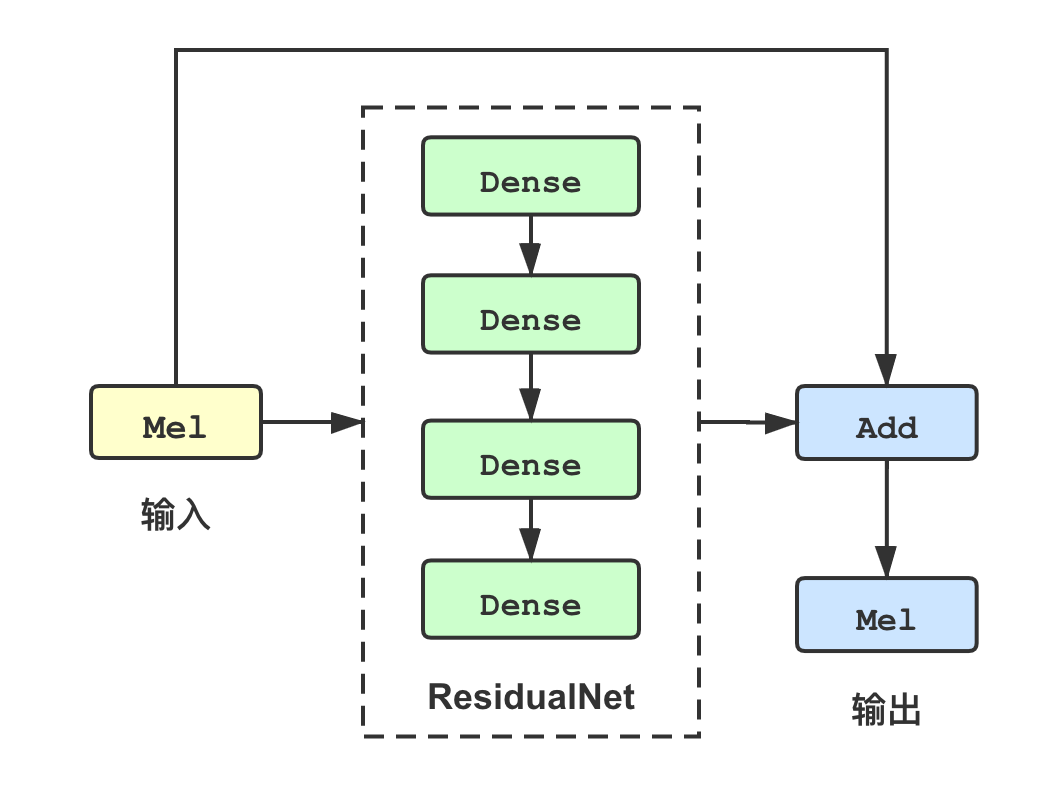
\includegraphics[width=.75\linewidth]{ResNet.png}
  \caption{ResidualNet 结构图}
  \label{fig:resnet}
\end{figure}

ResidualNet 的结构图如图 \ref{fig:resnet} 所示。

\section{探究残差网络对转换模型性能的影响($7"$)}

\textbf{(3)进行消融实验(Ablation Study),探究上述任务二中无残差网络的转换模型、与 本任务三中实现的有残差网络的转换模型的性能差别。}

\textbf{答:}

\begin{figure}[h]
\centering%
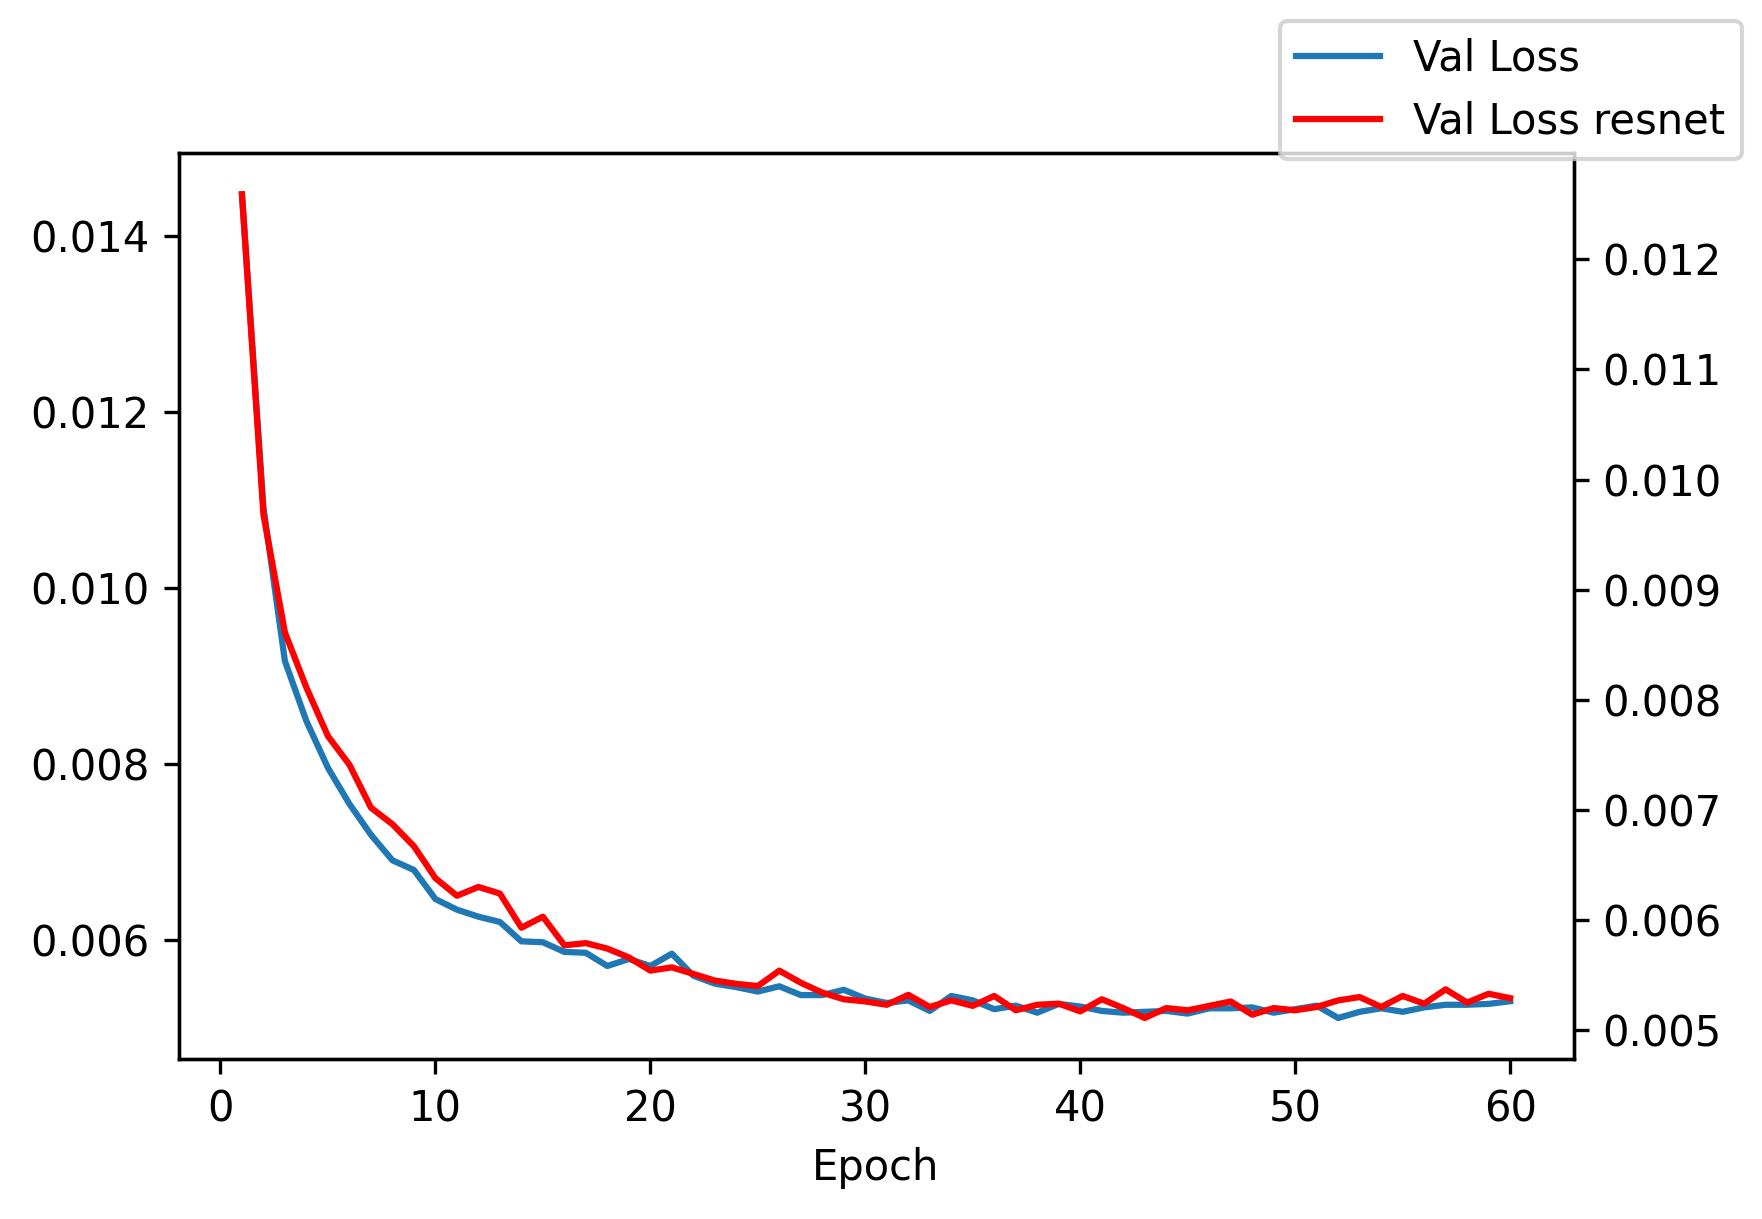
\includegraphics[width=.75\linewidth]{resnet_ablation.png}
  \caption{消融实验: 有无残差网络验证集结果对比}
  \label{fig:resnet_ablation}
\end{figure}

从 \ref{fig:resnet_ablation} 结果可以看出,有无残差网络的训练曲线基本一致。
对于最后一个 epoch 的验证集结果,有残差网络和无残差网络的损失值分别为 0.00529 和 0.00531,异有一点提升不过提升不显著。

至于实际的语音转换结果,使用 cmu\_us\_awb\_arctic/wav/arctic\_b0007.wav 作比较,感觉这两种模型的结果听起来没什么差别。

\chapter{任务四: 增加说话人嵌入网络,实现多目标说话人的语音转换($20"$)}

以上三个任务实现了一个多对一的语音转换(any-to-one VC)模型,本任务将在此基础上,通过增加说话人嵌入网络的结构,构建包含说话人嵌入网络的多对多的语音转换(any- to-many VC)模型,从而实现支持多个目标音色的多目标说话人的语音转换系统。
为了实现说话人嵌入网络,一个简单的办法就是给定说话人的 one-hot 标签,通过一个嵌入映射表(Embedding Table)得到该说话人对应的嵌入向量(Speaker Embedding),然后再通过一个全连接层,将全连接层输出与原有 DBSLTM 的两个 BLSTM 层的输入叠加,以此在原有的基于 DBSLTM 的转换模型中引入说话人信息,实现多说话人的转换模型。

\section{准备训练数据:提取多说话人的 PPG 及 Mel 谱等声学参数($3"$)}

\textbf{(1)根据 GitHub repository 的说明文档中的要求(Any-to-Many → Feature Extraction), 运行相关命令进行特征提取。请注意对提取的特征中的异常数据进行检查与去除,尤其需要 注意提取的特征数据中是否出现 NaN,若出现需要将相应的数据条目从*.csv 中删掉。}

\textbf{答:}

执行命令即可:

  \begin{minted}[texcomments,tabsize=2,fontsize=\footnotesize,style=friendly,bgcolor=friendlybg]{bash}
mkdir cmu_arctic/all
CUDA_VISIBLE_DEVICES=2 TF_FORCE_GPU_ALLOW_GROWTH=true python \
preprocess.py --data_dir cmu_arctic --save_dir cmu_arctic/all
\end{minted}

结果保存在文件夹 \texttt{cmu\_arctic/all} 中。

\section{实现说话人嵌入网络($9"$)}

\textbf{(2)根据说话人嵌入网络的有关原理,确定说话人嵌入网络的某种特定结构(鼓励探索更好的模型结构),并实现 models/model.py 中 SPKEmbedding 类的具体代码;如果有需要,可进一步对 models/model.py 中 BLSTMToManyConversionModel 类的相应部分进行修改。}

\textbf{答:}

代码如下所示,就是直接使用 PyTorch 的 Embedding 就好啦。

  \begin{minted}[texcomments,tabsize=2,fontsize=\footnotesize,style=friendly,bgcolor=friendlybg]{python}
class SPKEmbedding(nn.Module):
    def __init__(self, num_spk, embd_dim):
        super(SPKEmbedding, self).__init__()
        self.embedding_table = nn.Embedding(num_spk, embd_dim)

    def forward(self, spk_inds):
        return self.embedding_table(spk_inds)
\end{minted}

\textbf{(3)在实验报告中说明所实现的 SPKEmbedding 的具体结构,并给出网络的基本结构图。}

\textbf{答:}

SPKEmbedding 是一个形状为 $(n, D)$ 的矩阵,其中 $n$ 为说话人的个数,在本实验中就是 $6$ 啦。
然后 $D$ 是嵌入的维度,有超参数 \texttt{hps.BLSTMToManyConversionModel.spk\_embd\_dim} 控制,默认为 $64$。
假设嵌入矩阵为 $W$,对于输入的独热(one-hot)向量 $x$,输出嵌入就相当于 $W^Tx$,只不过因为 $x$ 很特殊,只有一个位置上的值为 1,其他位置上都是 0。
这样一般实现都是把 Embedding 实现为查找表,也就是直接按 $x$ 为 1 的那个位置的序号去找嵌入矩阵的那一行就好啦。

\textbf{(4)若对 BLSTMToManyConversionModel 类进行了修改,也需要在实验报告中加以说明。}

\textbf{答:}

BLSTMToManyConversionModel 类主要修改了 forward 函数,代码如下:

  \begin{minted}[texcomments,tabsize=2,highlightlines={3,5},fontsize=\footnotesize,style=friendly,bgcolor=friendlybg]{python}
def forward(self, x, spk_inds):
        spk_embds = self.spk_embed_net(spk_inds)
        blstm1_inputs = x + self.emb_proj1(spk_embds) # give your implementation here
        blstm1_outs, _ = self.blstm1(blstm1_inputs)
        blstm2_inputs = blstm1_outs + self.emb_proj2(spk_embds) # give your impl here
        blstm2_outs, _ = self.blstm2(blstm2_inputs)
        outputs = self.out_projection(blstm2_outs)
        return outputs
\end{minted}

\section{多目标说话人转换模型训练、验证、测试($4"$)}

\textbf{(5)根据 GitHub repository 的说明文档中的要求(Any-to-Many → Train),运行相关命令进行模型训练。}

\textbf{答:}

训练命令为:

  \begin{minted}[texcomments,tabsize=2,fontsize=\footnotesize,style=friendly,bgcolor=friendlybg]{bash}
env CUDA_VISIBLE_DEVICES=2 TF_FORCE_GPU_ALLOW_GROWTH=true stdbuf -o 0 python \
train_to_many.py --model_dir ./model_dir --test_dir ./test_dir \
--data_dir cmu_arctic/all 2>&1 | tee train_to_many.log
\end{minted}


\textbf{(6)给出模型训练时的损失函数曲线;模型训练了多少个 epoch?训练完成后,最终 (对应最后一个 epoch)的平均训练 MSE loss 是多少?}

\textbf{答:}

\begin{figure}[h]
\centering%
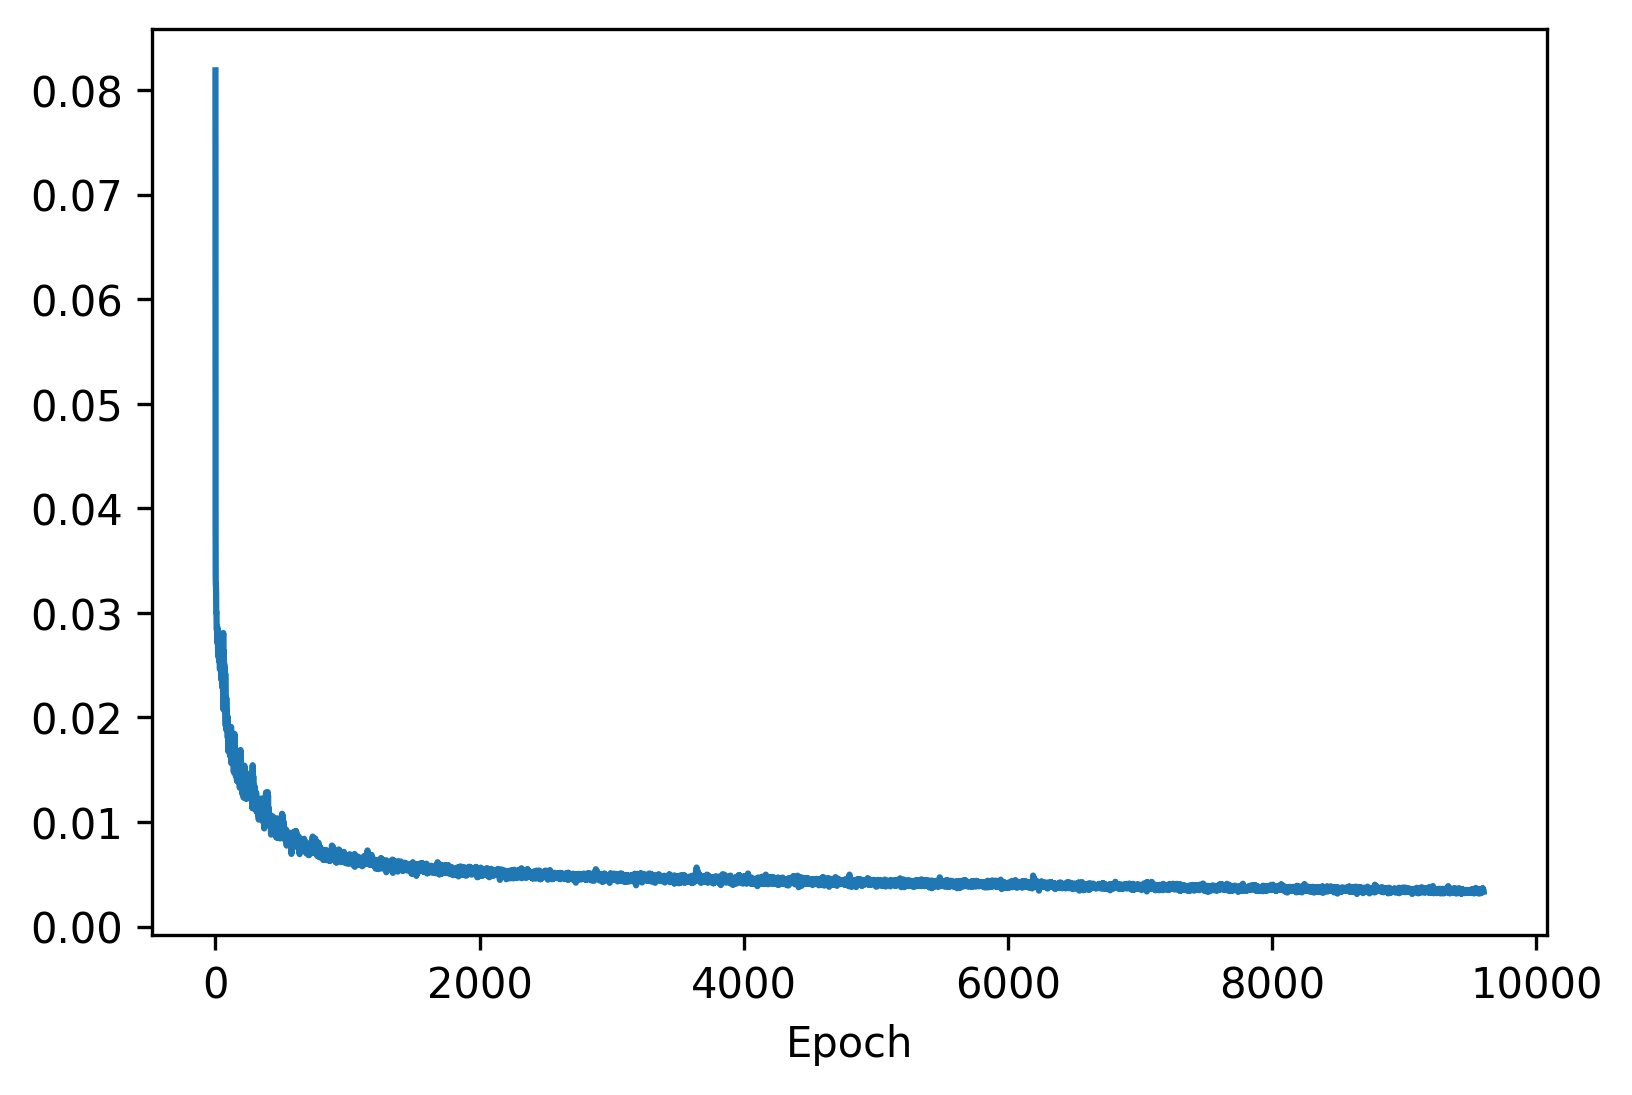
\includegraphics[width=.75\linewidth]{train_task4.png}
  \caption{多目标 VC 训练集损失曲线}
  \label{fig:train_task4}
\end{figure}

总共训练了 50 个 epoch,最终的平均训练 MSE loss 为 $0.00339$.

\textbf{(7)基于上述训练好的模型,在验证集上进行验证。在验证集上的 MSE loss 是多少?}

\textbf{答:}

\begin{figure}[h]
\centering%
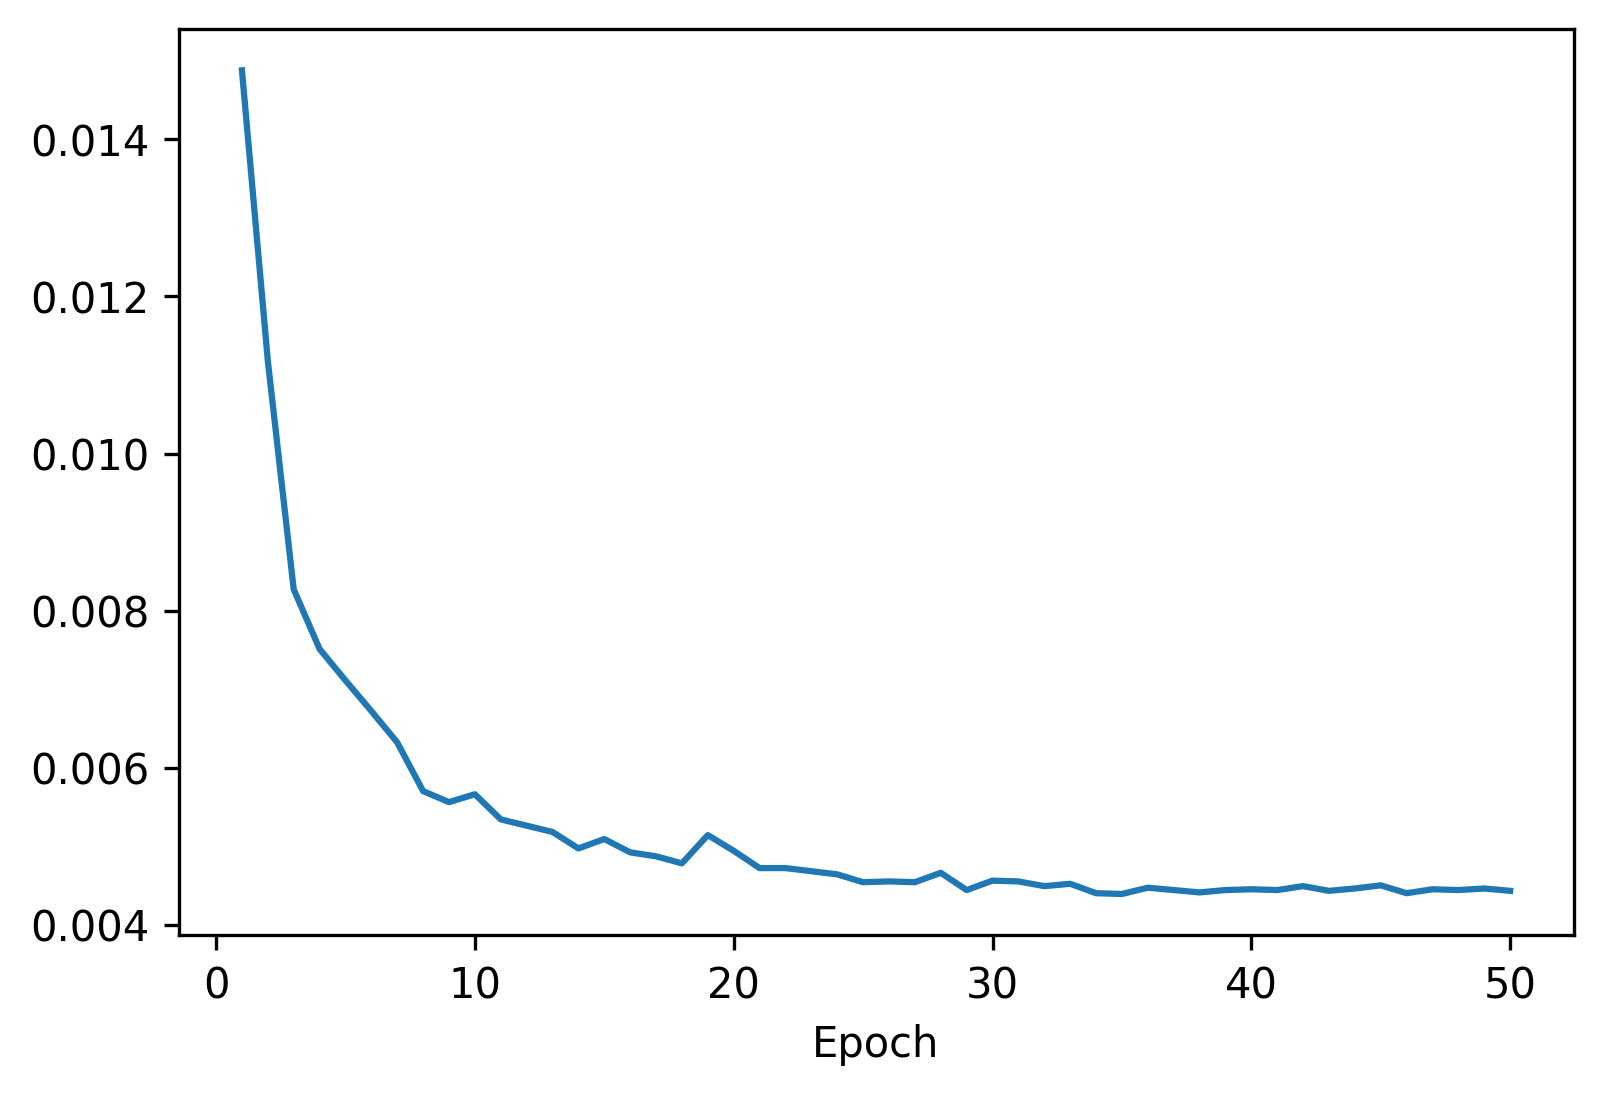
\includegraphics[width=.75\linewidth]{val_task4.png}
  \caption{多目标 VC 验证集损失曲线}
  \label{fig:val_task4}
\end{figure}

多目标 VC 验证集损失曲线如图\ref{fig:val_task4}所示,最终验证集的 MSE loss 为 $0.00443$。

\textbf{(8)基于上述训练好的模型,在测试集上进行测试。针对某句测试用例,通过给定不同的目标说话人的 Speaker ID,得到同一个源说话人的语音对应的不同目标说话人的转换语音;听辨转换语音的音色与目标说话人的音色,是否存在差异?为什么?}

\textbf{答:}

代码:

  \begin{minted}[texcomments,tabsize=2,fontsize=\footnotesize,style=friendly,bgcolor=friendlybg]{bash}
for tgt in slt bdl clb jmk rms; do 
CUDA_VISIBLE_DEVICES=0 TF_FORCE_GPU_ALLOW_GROWTH=true python inference_to_many.py \
--src_wav cmu_arctic/cmu_us_awb_arctic/wav/arctic_b0007.wav \
--tgt_spk $tgt --ckpt ./model_dir/ppg-vc-to-many-49.pt --save_dir ./demo_files/any-to-many
done
\end{minted}

为了和之前两个任务对比,依然选用 \texttt{cmu\_arctic/cmu\_us\_awb\_arctic/wav/arctic\_b0007.wav} 文件,转化为五种不同的说话人,结果输出保存在 demo\_files/any-to-many/中。
对比这些结果,我发现女声要比男声效果更加好一点,同时这五种声音在内容和说话人的特征上都很明显是成功转换了。
不过问题还是在于又一点电音,而且听起来也不是很清晰。

\section{进行多目标说话人语音转换($4"$)}

\textbf{(9)根据 GitHub repository 的说明文档中的要求(Any-to-Many → Inference),将某个特定源说话人的语音(src\_wav 参数)转换为某个特定目标说话人(tgt\_spk 参数)的语音。}

\textbf{答:}


通过修改参数 \texttt{tgt\_spk} 既可完成。
不足之处在于,声音听起来很容易发现是机器合成的,因为听起来不是很自然顺滑。

代码:
  \begin{minted}[texcomments,tabsize=2,fontsize=\footnotesize,style=friendly,bgcolor=friendlybg]{bash}
CUDA_VISIBLE_DEVICES=0 TF_FORCE_GPU_ALLOW_GROWTH=true python inference_to_many.py \
--src_wav cmu_arctic/cmu_us_awb_arctic/wav/arctic_b0007.wav \
--tgt_spk jmk --ckpt ./model_dir/ppg-vc-to-many-49.pt --save_dir ./demo_files/any-to-many
\end{minted}


\textbf{(10)自己录制一段语音,并作为模型的输入(src\_wav 参数),对 CMU\_ARCTIC 中的 6 个目标说话人(改变 tgt\_spk 参数)进行语音转换,得到 6 个转换后的语音。}

\textbf{答:}

  \begin{minted}[texcomments,tabsize=2,fontsize=\footnotesize,style=friendly,bgcolor=friendlybg]{bash}
for tgt in slt bdl clb jmk rms; do 
CUDA_VISIBLE_DEVICES=0 TF_FORCE_GPU_ALLOW_GROWTH=true python inference_to_many.py \
--src_wav my_test.wav \
--tgt_spk $tgt --ckpt ./model_dir/ppg-vc-to-many-49.pt --save_dir ./demo_files/any-to-many
done
\end{minted}



% 其他部分
\backmatter

% 参考文献
\bibliography{ref/refs}  % 参考文献使用 BibTeX 编译

% 附录
\appendix

\chapter{文件清单}

\begin{table}[htb]
  \centering
  \caption{文件清单}
  \label{tab:files}
  \begin{tabular}{cc}
    \toprule
    \textbf{文件(夹)}         & \textbf{说明}  \\
    \midrule
    \texttt{report.pdf} & 课程报告 PDF 文件 \\
    \texttt{source/report}           & 课程报告 LaTeX 源文件 \\
    \texttt{source/lab3.mb}        & 各个任务的命令执行过程 \\
    \texttt{source/dpss/logs} & 各个任务的训练日志 \\
    \texttt{source/dpss/models} & 修改后的模型 \\
    \texttt{source/dpss/demo\_files} & 各个任务的测试音频文件结果 \\
    \texttt{source/dpss/train\_to\_one\_resnet.py} & 训练 Any-to-one VC with ResNet 的代码 \\
    \bottomrule
  \end{tabular}
\end{table}

\end{document}